\documentclass[11pt, oneside]{article}   	% use "amsart" instead of "article" for AMSLaTeX format
\usepackage{geometry}                		% See geometry.pdf to learn the layout options. There are lots.
\geometry{letterpaper}                   		% ... or a4paper or a5paper or ... 
%\geometry{landscape}                		% Activate for rotated page geometry
%\usepackage[parfill]{parskip}    		% Activate to begin paragraphs with an empty line rather than an indent
\usepackage{graphicx}				% Use pdf, png, jpg, or eps§ with pdflatex; use eps in DVI mode
								% TeX will automatically convert eps --> pdf in pdflatex		
\usepackage{amssymb}

\usepackage{tikz}
\usetikzlibrary{arrows}
\usetikzlibrary{decorations.markings}


%SetFonts

%SetFonts


\title{Brief Article}
\author{The Author}
%\date{}							% Activate to display a given date or no date

\begin{document}
\maketitle
%\section{}
%\subsection{}

This is a test file.

\begin{table}[htbp]
	\centering
	\begin{tabular}{r|c|l||}
	a & b & c \\
	d & e & f \\
	a & & \\
	\hline
	\end{tabular}
	\caption{caption}
	\label{label}
\end{table}
$$\int_2^3 f(x) dx = 15$$
\begin{center}
	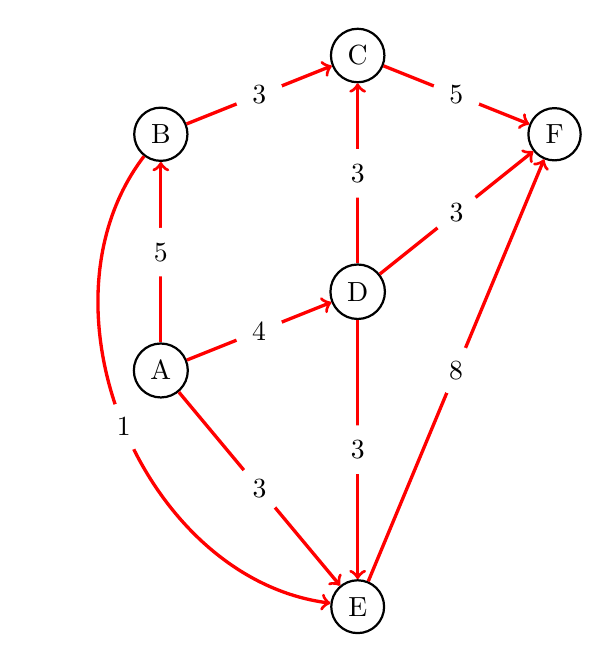
\begin{tikzpicture}
		\begin{scope}[every node/.style={circle,thick,draw}]
			\node (A) at (0,0) {A};
			\node (B) at (0,3) {B};
			\node (C) at (2.5,4) {C};
			\node (D) at (2.5,1) {D};
			\node (E) at (2.5,-3) {E};
			\node (F) at (5,3) {F} ;
		\end{scope}
		
		\begin{scope}[,
					  every node/.style={fill=white,circle},
					  every edge/.style={draw=red,very thick}]
			\path [->] (A) edge node {$5$} (B); 
			\path [->] (B) edge node {$3$} (C);
			\path [->] (A) edge node {$4$} (D);
			\path [->] (D) edge node {$3$} (C);
			\path [->] (A) edge node {$3$} (E);
			\path [->] (D) edge node {$3$} (E);
			\path [->] (D) edge node {$3$} (F);
			\path [->] (C) edge node {$5$} (F);
			\path [->] (E) edge node {$8$} (F); 
			\path [->] (B) edge[bend right=60] node {$1$} (E); 
		\end{scope}
	\end{tikzpicture}
\end{center}

\section{Chapter 1}

Hello


\section{Chapter 2}
Yay
\subsubsection{Subsection 1}
Some Notes

% More complicated graph with edge weights

\begin{tikzpicture}

	\tikzset{vertex/.style = {shape=circle,draw,minimum size=1.5em}}
	\tikzset{edge/.style = {->,> = latex'}}
	% vertices
	\node[vertex] (a) at  (0,0) {};
	\node[vertex] (b) at  (4,3) {};
	\node[vertex] (c) at  (8,0) {};
	\node[vertex] (d) at  (4,-3) {$t$};
	\node[vertex] (a1) at (1.5,0) {};
	\node[vertex] (a2) at (3,0) {};
	%edges
	\draw[edge] (b) to (a);
	\draw[edge] (b) to (c);
	\draw[edge] (a) to (d);
	\draw[edge] (c) to (d);
	
	\draw[edge] (a)  to[bend left] (a1);
	\draw[edge] (a1) to[bend left] (a);
	
	\draw[edge] (a1) to[bend left] (a2);
	\draw[edge] (a2) to[bend left] (a1);
	
	\path (a2) to node {\dots} (c);
	\node [shape=circle,minimum size=1.5em] (a3) at (4.5,0) {};
	\draw[edge] (a2) to[bend left] (a3);
	\draw[edge] (a3) to[bend left] (a2);
	
	\node [shape=circle,minimum size=1.5em] (c1) at (6.5,0) {};
	\draw[edge] (c) to[bend left] (c1);
	\draw[edge] (c1) to[bend left] (c);
\end{tikzpicture}


% Adding Center Arrow Marking Decoration

\tikzset{->-/.style={decoration={
  markings,
  mark=at position #1 with {\arrow{latex}}},postaction={decorate}}}

\begin{tikzpicture}
 \draw[->-=.5, very thick] (0,0) to [bend left] (2,4);
 \draw[->-=.8, thick] (0,0) to [bend right] (2,4);
\end{tikzpicture}
	

\end{document}  